% title page
\linespread{1.0}\selectfont
\thispagestyle{empty}
\pagenumbering{gobble}
\selectlanguage{ngerman}
\pdfbookmark[1]{Titlepage}{Titlepage}
\renewcommand{\headrulewidth}{0pt}
\begin{center}
	\vspace*{2cm}

	\begin{spacing}{1.8}
		\textsc{\LARGE \title}\\
	\end{spacing}

	\vspace{1.5cm}

	von\\

	\vspace{1.5cm}

    {\large \author}\\

	\vspace{1.5cm}

	vorgelegt der\\
    Fakultät für Mathematik, Informatik und Naturwissenschaften \\
    RWTH Aachen

	\vspace{0.25cm}

%	{\large PREVIOUS QUALIFICATION}\\

	\vspace{0.5cm}

%	aus HOMETOWN\\

	\vspace{1.5cm}

	\begin{tabular}{rl}
		Berichter: & Universit\"atsprofessor \profprim\\
		& Universit\"atsprofessor \profsec\\
	\end{tabular}\\

	\vspace{1.5cm}

	Datum der m\"undlichen Pr\"ufung: \defensedate\\

	\vfill

\end{center}

\newpage

\null

\vfill

\textbf{\author}\\
\textsc{\title}\\

\textbf{Masterarbeit in Physik}\\
Rheinisch-Westf\"alische Technische Hochschule Aachen\\
III. Physikalisches Institut A\\

\begin{tabular}{@{}ll}
\textbf{Berichter}: & Universit\"atsprofessor \profprim\\
& Universit\"atsprofessor \profsec\\
\end{tabular}


% contents page
\newpage
\pagenumbering{Roman}
\setcounter{page}{1}
\thispagestyle{fancy}
\fancyhead{}
\fancyfoot{}
\fancyfoot[RO,LE]{\slshape{\thepage}}
\selectlanguage{english}
\pdfbookmark[1]{Contents}{Contents}
\addtocontents{toc}{~\hfill\textbf{Page}\par}
\tableofcontents

% begin thesis content
%\pageshift
\pagenumbering{arabic}
\setcounter{page}{1}
\linespread{\textlinespread}\selectfont
\fancyfoot[RO,LE]{\slshape{\thepage}}
\fancyhead[LE]{\slshape{\leftmark}}
\fancyhead[RO]{\slshape{\rightmark}}
\renewcommand{\headrulewidth}{0.5pt}

% introduction
%\thispagestyle{plain}
%\Section{Introduction}
\label{sec:introduction}

The discovery of the Higgs boson by the CMS and ATLAS experiments at the Large Hadron Collider in 2012 has opened frontiers towards new physical phenomena \cite{Chatrchyan_2012}. As the Standard Model of Particle Physics (SM) is incomplete, precision measurements in the Higgs sector are promising candidates for Beyond the Standard Model model-limiting measurements. It has been proposed that the ratio of cross sections of the gluon fusion induced ZH final states to the quark induced ZH production is a sensitive observable towards such phenomena \cite{Harlander_2018}. As the direct extraction of the gluon fusion induced process is limited by current experimental setup and analysis techniques due to the destructive interference of the contributing diagrams, the quark induced WH production cross section is included in the proposed measurement.

Newly developed deep learning methods have shown great success in analytically unsolvable tasks such as image classification, generation and captioning, text translation, -generation and regression tasks \cite{LeCun2015}. In a particle physics context, they have become a powerful tool for jet-flavour identification, pileup mitigation, detector effect simulation and process classification \cite{Schwartz_2021}. Most of these modern approaches are built upon neural networks and tackle the challenge of posterior inference by data-driven methods.

Conditional invertible neural networks have already proven to be successful in guided image generation and -colorization \cite{cINN_im_gen} and stochastic model learning \cite{BayesFlow}. Thanks to their invertible nature, these networks can infer the posterior distributions of the underlying model parameters directly. In physics, these networks have proven to be successful in their application to stellar parameter estimation \cite{Ksoll_2020}, cosmic ray source property inference \cite{Bister_2022} and detector effect simulation \cite{Bellagente_2020}.

The continuous growth in model complexity in high energy physics demands increasingly time-consuming likelihood fits. In this thesis inference of signal strength modifiers and nuisance parameters with cINNs will be discussed. Upon successful training, these networks can infer the physics parameters quickly and for low computational cost. The performance measures of the resulting network will be characterized and discussed in detail.

This thesis is structured as follows: ch. \ref{ch:theory} describes the Standard Model and the signal processes for which the signal strength parameters will be inferred. Ch. \ref{ch:experiment} discusses the experimental setup. In ch. \ref{ch:deeplearning}, the foundations of deep learning and conditional invertible neural networks are introduced with a focus on the resulting network setup. Ch. \ref{ch:analysis_strategy} describes the analysis strategy and -setup. The cINN models are described in ch. \ref{ch:network_setup}. Last, the predictions and the performance measures are discussed in \ref{ch:inference}.

% theory
\pageshift
\thispagestyle{plain}
\Section{Experimental Setup}

In this chapter the experimental context of this thesis will be discussed. 

\Subsection{The Large Hadron Collider}
\label{sec:theory}

The Large Hadron Collider (LHC) is currently the most powerful particle accelerator in the world. Hosted at CERN in Geneva at the Swiss-French border and first put into operation on $\text{10}^\text{th}$ September 2008, the LHC is designed for proton and heavy lead ion collisions. The machine has gone through several upgrades between the consecutive data-taking phases (Runs) called Long Shutdowns (LS). During these the proton beam energy has been gradually increased from \SI{3.5}{\tera\electronvolt} to a recently -- on the $\text{5}^{\text{th}}$ July, 2022 to be precise -- achieved energy of \SI{6.8}{\tera\electronvolt} \cite{Alici:2773265} resulting in a total centre-of-mass (CM) proton-proton collision energy of $\sqrt{s} = \SI{13.6}{\tera\electronvolt}$. Similarly, the beam intensity has seen an increase from $1.1 \times 10^{11}$ protons per bunch (ppb) and $\sim 200$ bunches to a projected $\sim1.8 \times 10^{11}$ ppb and $\sim2500$ bunches \cite{Fartoukh:2790409, Karastathis:2750302}. With a theoretical maximum CM energy of $\sqrt{s} = \SI{14}{\tera\electronvolt}$ and integrated luminosity of $L = \SI{10d34}{\centi\meter^{-2}\second^{-1}}$ it holds the record in these measures among concurring experiments. In order to achieve such luminosities, the beams are kept on a circular trajectory using superconducting NbTi magnets operating at \SI{1.9}{\kelvin} thanks to the superfluid helium bath at about \SI{0.13}{\mega\pascal} \cite{Brüning:782076}.

As a result of consecutive accelerator upgrades, the collider complex has an impressive and complex pre-accelerator structure as shown in fig. \ref{fig:lhcstructure}. Consequently, the proton bunches first go through multiple preparation steps before they get injected into the \SI{27}{\kilo\meter} tunnel of the LHC where the four main experiments (ALICE, ATLAS, LHCb and CMS) and their interaction points are located. 

\begin{figure}[h!]
	\centering
	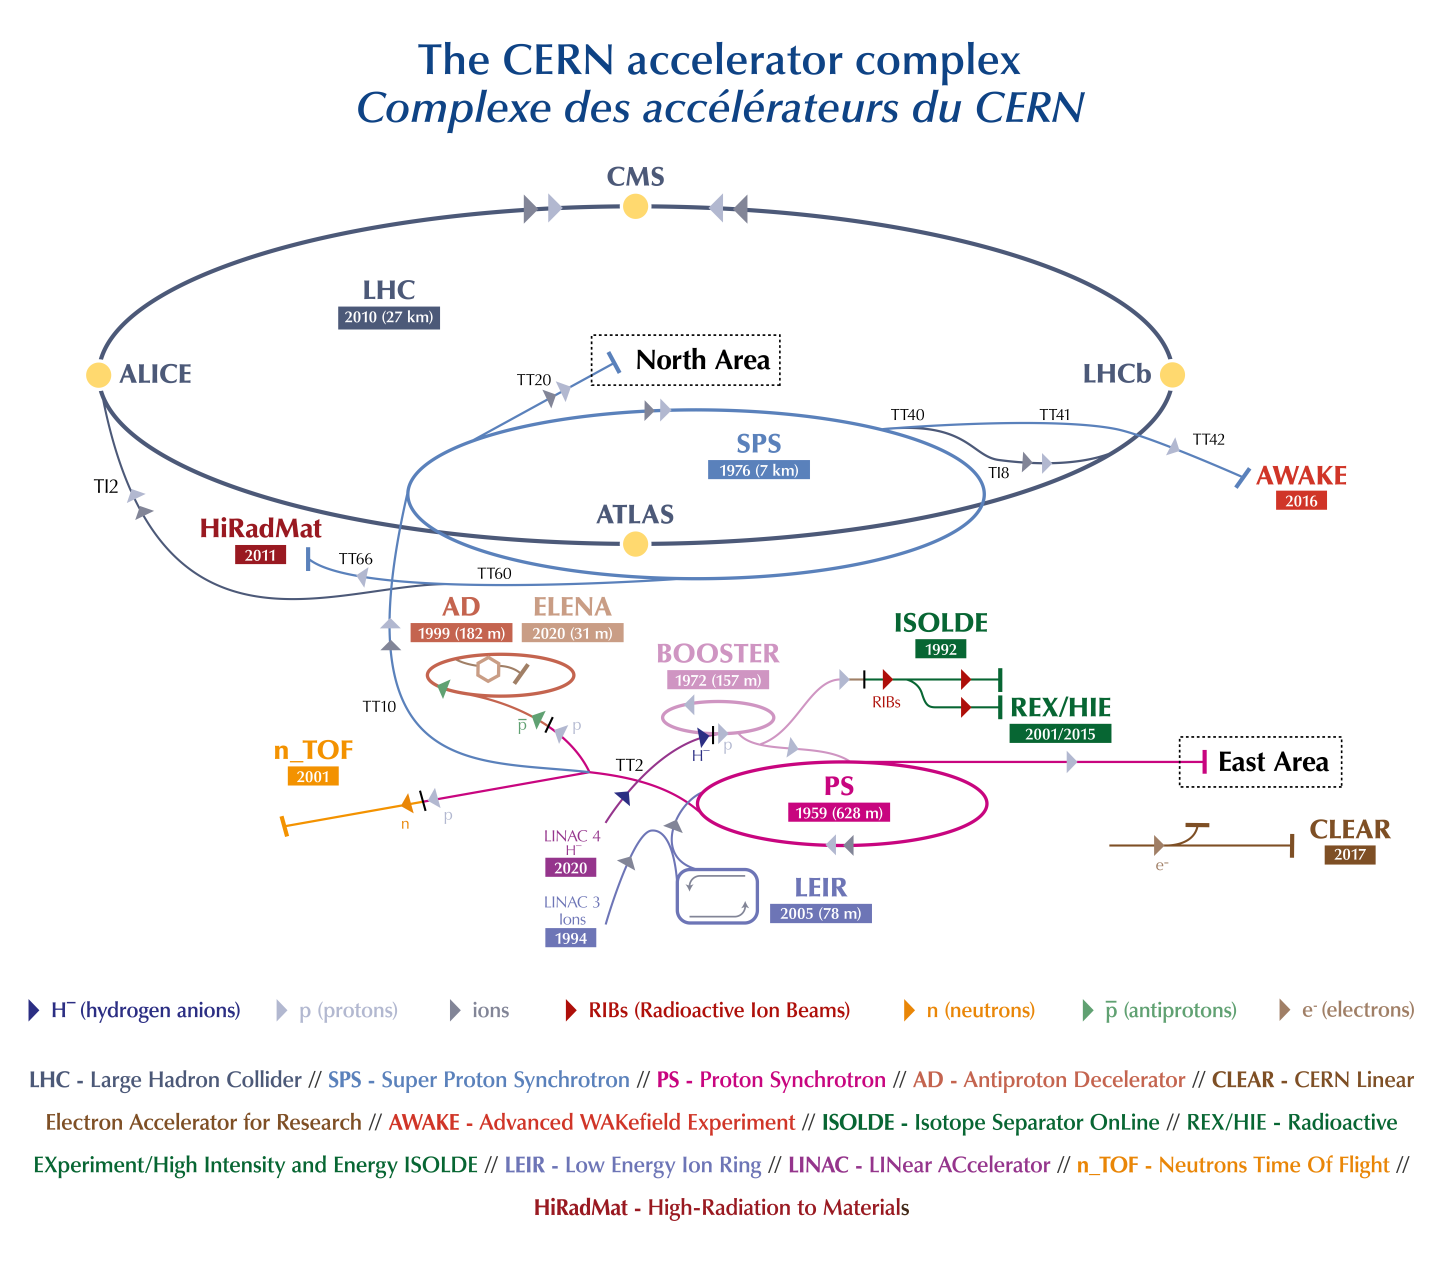
\includegraphics[width=\textwidth]{figures/theoryexperiment/CCC-v2019-final-white}
	\caption{The pre-accelerator complex of the LHC and their corresponding construction years. Accelerator and storage rings are shown in different colours, the particles they accelerate are shown as arrows. Note that the pre-acceleators do not serve the LHC ring exclusively and the diverging paths lead to other independent experiments. Old tunnels of previous experiments serve as pre-accelerators now in the LHC injection chain. \cite{Mobs:2684277}}
	\label{fig:lhcstructure}
\end{figure}

The four main stages of pre-acceleration for protons are listed in \ref{tab:preaccelerators} below. As proton source, hydrogen is used. The protons are first accelerated in the form of H$^-$ ions through the 86 metre long tunnel of the recently (2020) constructed Linear Accelerator 4 (Linac4). Stripped of their pair of electrons, the protons enter the Proton Synchrotron Booster (PSB) where they reach up to \SI{2}{\giga\electronvolt}. In the next step of the injection chain, they enter the Proton Synchrotron (PS), historically the first synchrotron at CERN serving exclusively as a pre-accelerator now. Travelling through the 628 metre long ring and accelerated to 26 GeV, the particles are injected into the Super Proton Synchrotron (SPS), where they are awaiting injection into the LHC once they reach 450 GeV.

\begin{table}[h!]
	\centering
	\begin{tabular}{c|c}
		Accelerator & Peak Energy \\
		\hline
		\hline
		Linear accelerator 4 (Linac4) & 160 MeV \\
		\hline
		Proton Synchrotron Booster (PSB) & 2 GeV \\
		\hline
		Proton Synchrotron (PS) & 26 GeV \\
		\hline
		Super Proton Synchrotron (SPS) & 450 GeV \\
		\hline
		Large Hadron Collider (LHC) & 7 TeV \\
	\end{tabular}
	\caption{The acceleration chain the protons undergo to reach their final energy of 7 TeV.}
	\label{tab:preaccelerators}
\end{table}

\color{red}{Entering the LHC, they live happily forever after until they are brutally crushed into each other and die of quantum mechanics.}\color{black}



\Subsection{The Compact Muon Solenoid}

One of general purpose detectors at the Large Hadron Collider at CERN is the Compact Muon Solenoid (CMS).


% other sections go here

% conclusion
\pageshift
%\thispagestyle{plain}
%\Section{Conclusion}
\label{sec:conclusion}

Since its discovery in 2012, the continuous research on the Standard Model (SM) Higgs boson has proven to be a fruitful endeavour. In order to constrain the Beyond the Standard Model nature of its coupling to known SM particles, several SM testing measurements have been performed, some of which require innovative analysis techniques.\\

In this thesis, inference on signal strength modifier parameters with cINNs at the CMS experiment has been discussed in detail. Thanks to their unique feature of being able to infer the true posterior distribution conditioned on observables directly, these networks are capable of reconstructing physics parameters correctly. In addition to that, Bayesian inference upon successful training takes several orders of magnitude less time than model fits based on frequentist approaches. Several proposed novel analysis approaches require the gradient of the observables to be propagated by such networks; as cINNs are built upon normalizing flows, the diffeomorphism encoded in the network model fulfils this property.\\

The gluon-fusion induced ZH production channel is a suitable candidate to look BSM effects for due to the loop-induced nature of the process at leading order. Using the measurable cross section of the quark initiated ZH and WH production processes, the observable $R^{ZW}_R$ can be measured by extracting the three signal processes from data via a likelihood fit.\\

In has been shown that the signal strength modifier parameters obtained from the likelihood fit can be inferred by the cINN model. Inference has been performed on the DNN probability scores for the three signal processes, 13 background nuisance parameters and one normalizing uncertainty, the luminosity. With that, the resulting network model had 17 dimensional inputs of physics parameters and a 235 dimensional condition input as physics observables on which the posteriors are conditioned on.

The study has been performed on simulated events exclusively. The training data has been constructed to reflect the expected statistical and systematic effects in measured data. For the former, both the limited MC sample size and the expected Poisson effects in the data have been taken into account. The shape-changing systematic effects are computationally expensive to simulate. For this reason, a non-linear histogram interpolation method (morphing) has been implemented to inter- and extrapolate among histogram templates. \\

Upon training, inference has been performed on the SM expectation. The obtained values for the signal process were

\begin{equation*}
		\mu_\text{ggZH} = 5.10^{+3.57}_{-3.50}, \, \, \quad \mu_\text{ZHDY} = 3.90^{+2.62}_{-2.57}, \, \, \quad \mu_\text{WH} = 3.02^{+1.92}_{-1.90} 
\end{equation*}

The sensitivity of the network with respect to different signal regions and physics processes has been discussed in detail. It has been shown that the network model does not have inherent biases due to wrong initialization or training relics. Rather, the network returns broad posteriors in regions of low sensitivity as expected. In addition to that, the network returns the prior distribution for unrecognized processes. It has been noted that the network cannot be more sensitive then the analysis itself.

% appendix
%\begin{appendix}
%	% appendix sections should look like this
%	 \pageshift
%	 \thispagestyle{plain}
%	 \Section{Foo}\label{sec:apx_foo}
%	 Foo.
%\end{appendix}


% bibliography
\linespread{1.0}\selectfont
\pageshift
\thispagestyle{plain}
\renewcommand{\headrulewidth}{0pt}
\renewcommand{\refname}{Bibliography}
\phantomsection
\addcontentsline{toc}{section}{Bibliography}
\bibliography{bib/bib}

% finalize thesis content
\renewcommand{\headrulewidth}{0pt}
\fancyhead{}
\fancyfoot{}

% thesis statement
\pageshift
\thispagestyle{empty}
\section*{Selbst\"andigkeitserkl\"arung}

Hiermit versichere ich an Eides statt, dass ich diese Arbeit einschlie\ss lich evtl. beigef\"ugter Abbildungen, Zeichnungen u.\"A.m. selbstst\"andig angefertigt und keine anderen als die angegebenen Hilfsmittel und Quellen benutzt habe. Alle Stellen, die dem Wortlaut oder dem Sinn nach anderen Werken entnommen sind, habe ich in jedem einzelnen Fall unter genauer Angabe der Quelle deutlich als Entlehnung kenntlich gemacht.\\
%
\vspace{1cm}
\\
{Aachen, den \handindate}\hfill
\begin{tabular}{c}
	\\\\\hline
	\hspace*{24mm}\author\hspace*{24mm}
\end{tabular}


% acknowledgment
\pageshift
\thispagestyle{empty}
\selectlanguage{ngerman}
\section*{Danksagung}

Thx.

